\subsection{Magnetic Field Interpolation} \label{ssec:val_magfield}

    \begin{figure}[ht]
        \centering
        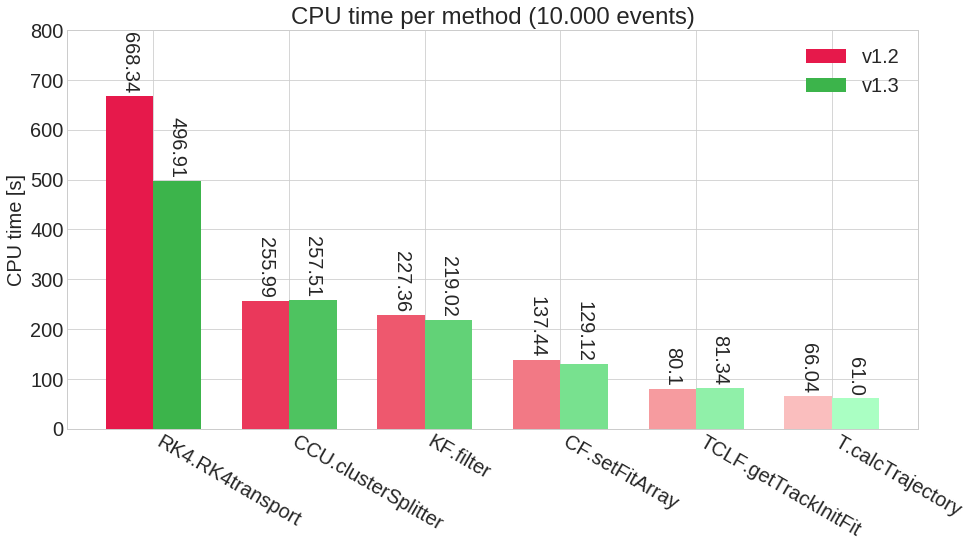
\includegraphics[scale=0.44]{methods_times/1_3}
        \caption{\label{fig:methods_times-1_3} Method CPU times, version $1.3$ compared with $1.2$.}
    \end{figure}
    
The time reduction brought by interpolating the magnetic field described in Section \ref{ssec:prop_magfield} was of $9.2\%$ (from $113.19$ to $102.79$ [ms]) per event for the DCHB engine, while no improvement was seen for DCTB because, as described in the subsection, it isn't considered affordable to lose precision in Time-Based tracking.

Figure \ref{fig:methods_times-1_3} clearly shows that the largest bulk of improvement was in the \texttt{RK4transport} method as should be expected, since this method calls the magnetic field methods that were slowing down the computation.
All the other changes in the different methods are attributed to random differences between the profiling sessions, which are to be expected considering that the profiling was done via statistical sampling, as described in Section \ref{sec:prof}.